% !TeX root = ../main.tex

\chapter{系統設計}
自主身份(AID)系統是一種創新的身份管理架構,其核心理念在於賦予個體對其身份資料的完全控制權。在這個系統中,三個關鍵角色相互協作:用戶、服務提供者和共識核心。用戶作為系統的終端使用者,通過個人設備全權管理自己的身份資料,根據需求選擇性地使用任意個服務並控制資料的流動。服務提供者則擔任用戶聚集的節點,不儲存用戶資料,而是根據用戶提供的資訊完成相應服務,並可靈活地根據實際場景客製化管理模式。共識核心則扮演著關鍵的中介角色,連接服務與服務、服務與用戶,提供用戶數據背書和信任評價機制,成為整個生態系統的基石。

本章節將深入探討此系統的架構設計、資料結構和潛在威脅模型,全面分析其如何在保障用戶自主權的同時,實現高效、安全的身份管理。
\section{系統的重要進步}
為實現用戶對其身份的完全自主權,本研究提出了多項創新機制,旨在解決現有的技術困境。
\subsection{別名優先機制}
傳統的身份驗證系統要求使用者提供唯一帳號作為登入識別。然而,這種設計無形中剝奪了用戶對個人名稱的自主權。一個連名稱都無法自主的系統,顯然難以達成本研究的設計目標。因此,我們提出讓用戶在註冊身份時優先使用自己喜歡的別名,再透過 UUID 機制\cite{uuid}產生唯一識別號。在日常操作中,系統優先讓用戶使用別名作為帳號,只有當別名因重複而難以識別時,才會要求用戶使用與 UUID 關聯的機制進行識別。當然,何時該使用別名,何時該使用 UUID,這是個複雜的問題。為此,我們提出了「基於用戶時空的分析方法」,試圖系統性地進行分析。
\subsection{基於用戶時空的分析方法}
每個身份本質上可視為一個隨時間變化的動態向量空間,其維度可謂無窮。每次對用戶的身份驗證都可視為取得特定時間僅含部分維度的向量。這方法的核心是讓用戶自主決定提供哪些維度,並在每次與系統互動時攜帶這些資訊。基於此概念,系統可藉由比對當次傳入的向量和近期暫存在快取中的所有向量來推測用戶的真實身份。

舉例來說:用戶在某次登入時提供了自己的別名、性別、所在地區等資訊,而在下次登入時僅提供了性別、所在地區等資訊,系統可以通過比對這兩次向量來推測用戶的別名。這種方法使用戶在不提供完整資訊的情況下,仍能通過部分資訊完成身份驗證。

然而,這種方法也帶來了一些問題。例如,用戶提供的維度多寡會影響系統的準確性,甚至用戶提供的維度是否包含可變資訊會影響系統的安全性。因此,我們提出維度的選擇甚至各個維度的權重應由用戶自主決定,而系統僅提供推薦機制。這樣可讓用戶在不同情境下使用不同方法,以滿足其需求。

總的來說,當僅有一個用戶被比較出來時視為可識別,有零個或多個用戶被比較出來時視為不可識別。這種機制受比較方法影響,因此我們提出了「基於危險程度的驗證機制」,希望能在不同情境下選擇適合的比較方法。
\subsection{基於危險程度的驗證機制}
此機制主要使用在比較身份與歷史紀錄時選擇適合的比較方法。不同的比較方法可能導致不同的結果,因其本質上代表了不同的嚴謹程度。在嚴謹程度較高的情況下,用戶可能需要更多維度符合,或需要在更接近的時間點內提供的紀錄才算數。這可能導致用戶難以找到識別對象,進而要求補充更多資訊再次驗證。相反,在嚴謹程度較低的情況下,用戶可能僅用少量維度的資訊配合較遠時間點的紀錄來完成驗證,這可能導致用戶被誤認為其他用戶,威脅系統安全。

考慮用戶行為的危險程度,我們設計出以下規則:
\begin{enumerate}
  \item 當用戶的行為被視為危險時,系統應提高驗證的嚴謹程度。
  \item 當用戶的行為被視為安全時,系統應降低驗證的嚴謹程度。
\end{enumerate}

接著,我們將嚴謹程度拆分為時間和空間兩個軸,使用笛卡爾座標系統表示,以細分出更複雜的情境:
\begin{enumerate}
  \item 當用戶行為超危險時,比較標準應為時間非常近或多個維度符合。
  \item 當用戶行為危險時,比較標準應為時間相對近或維度相對符合。
  \item 當用戶行為安全時,比較標準應為時間相對遠或維度相對不符合。
  \item 當用戶行為超安全時,比較標準應為時間非常遠或僅幾個維度符合。
\end{enumerate}

最後,用戶行為的危險程度在我們的系統中是由用戶自主決定的,系統僅提供推薦機制。我們希望藉此滿足所有用戶在各種情境下的需求。例如,對於個人銀行帳戶,可能所有行為都視為最高危險,因此需要最高的驗證嚴謹程度。而對於個人社群帳戶,讀取文章的行為可能視為不危險,發布文章則視為危險,因此需要不同的驗證嚴謹程度。我們建議用戶將危險的概念定義為對用戶數據變動的敏感程度:越敏感的數據越危險,越危險的數據越需要嚴謹的驗證機制。
\subsection{極致多因素認證}
傳統身份驗證系統中,多因素認證被廣泛使用,但僅被視為登入時的驗證方案。然而,我們認為多因素中的每個因素都可視為一個維度,而這些維度可由用戶自主選擇。因此,我們提出了極致多因素認證的概念:我們認為不存在特定的多因素驗證方法作為用戶登入的唯一方式,而應該反過來,從服務器的角度觀察,每個因素的驗證應該是用戶向服務器自主證明自己身份的方法。

因此,在足夠危險的情況下,可能需要連續多種因素的驗證;而在足夠安全的情況下,可能只需要一種因素的驗證。甚至即便遺失了某個重要因素,也不應被視為無法登入,而應被視為需要提供更多其他因素的驗證。
\subsection{自主證書}
本研究提出了一種創新的基於區塊鏈技術的自主身份驗證流程,旨在解決傳統身份管理系統中使用者對身份驗證缺乏自主權的問題。在傳統模式下,使用者的身份驗證資訊通常由身份服務提供者集中管理,這種做法實質上限制了使用者對其個人身份資訊的控制權。為了解決這一問題,我們參考了Tze-Nan\cite{NTU202102846}提出的自主證書機制,設計了一個基於區塊鏈技術的新型身份管理流程。

本研究提出的身份管理流程包含以下關鍵步驟:
\begin{enumerate}
  \item 簽章證書:使用者可以針對相同的自主身份在不同的簽章者處建立不同目的的證書,其內提供不同數據與權限。
  \item 區塊鏈驗證:證書的簽名會被簽章者記錄在區塊鏈上,服務提供者可以在區塊鏈上查詢證書的真實性,確保身份資訊的可信度。
  \item 證書撤銷:使用者可以隨時撤銷證書,並在區塊鏈上提交撤銷的簽名。這種機制可以應用於證書外流等情況,提高系統的安全性和可靠性。
  \item 自主註冊:使用者在註冊時,主動向服務提供者提交自己的證書,表明自己的身份。
  \item 彈性驗證:使用者在進行身份驗證時,可以根據證書自主選擇多因素驗證(MFA)的方式,提高身份驗證的便利性和安全性。
\end{enumerate}
此外,本系統的證書機制支援多樣化的功能,進一步提升了使用者對其身份資訊的控制權:
\begin{itemize}
  \item 自定義多因素認證選項
  \item 選擇性資訊揭露
  \item 設置證書有效期限
  \item 指定特定的驗證條件 (如特定設備,地點或時間)
  \item 指定特定的驗證規則(設備和網路使用限制)
  \item 資源存取權限控制 (如檔案存取權限)
\end{itemize}

總結來說,通過這種機制提升了系統對用戶隱私和安全的保護程度,讓用戶能夠更自主地管理其身份驗證流程,保持對個人身份驗證的控制權。
\subsection{數據共識}
在傳統身分管理系統中,基於安全和隱私的考慮,資料孤島問題一直難以有效解決。自主身分系統的出現為此提供了解決方案。使用者可以使用個人設備儲存自己的身份訊息,並在加入另一個自主身份系統時選擇性地上傳部分資訊。但這種設計仍然無法徹底解決資料孤島問題。尤其是當使用者想要共享的資料價值較高且可能被更改時,例如資產證明,此類資料無法僅在使用者的個人裝置上儲存和操作。

為了解決這一問題,本研究提出了一種基於區塊鏈的共識機制。在這種機制中,每個自主身份服務可以在區塊鏈上提交針對特定使用者特定數據的校驗簽名,進而讓其他服務能夠驗證使用者特定數據的真實性。這種設計使用戶能夠在不同的自主身份服務中安全地共享資料,同時向其他用戶保證資料的一致性和可信度。

這種基於區塊鏈的共識機制不僅有效解決了數據孤島問題,還提供了多方面的優勢。首先,通過區塊鏈技術確保了數據的完整性,有效防止數據被篡改。其次,它實現了使用者在不同自主身份系統間的無縫數據共享。再者,這種機制仍然保護了使用者的隱私,讓使用者能夠控制哪些數據被共享,保持對個人資訊的自主權。最後,它還支援實時驗證,其他服務可以即時驗證使用者數據的真實性,無需複雜的跨系統認證流程。
\subsection{自主身份數據管理}
基於前文所述的「自主證書機制」與「數據共識機制」,我們發展出了「自主身份數據管理」方法,旨在徹底解決被遺忘權和積極數據授權等棘手的隱私問題。在自主身份框架下,用戶通過自有裝置保存個人數據,包括證書與資料。當用戶需要證明身份時,需依照「自主證書機制」上傳證書給服務提供者,以完成對用戶的信任與驗證。而當用戶需要使用數據時,則上傳本地的相關數據,並可透過「數據共識機制」使服務提供者信任用戶所提供數據的真實性。

此外,針對特殊的隱私問題,自主身份數據管理提供了以下解決方案:
\begin{itemize}
  \item \textbf{被遺忘權}:當用戶希望遺忘數據時,可直接清除個人保留的數據。區塊鏈中僅保留簽名,而不保留數據本身。理論上,服務內部不會存儲用戶數據;即使確實存儲了,由於唯一能證明數據擁有人的是用戶本身,因此相當於用戶與數據無關。這個概念類似於 Cameron\cite{cameron2005laws}所描述的單向身份:用戶可以通過個人證明指向自己的數據,但僅有數據無法指向用戶。
  \item \textbf{積極數據授權}:採用類似「自主證書」的方法,使用戶與服務提供者對數據授權產生明確共識。當用戶授權服務提供者使用數據時,會對數據與使用範圍生成證書,並上傳對應簽名至區塊鏈,然後將證書與數據傳送給服務提供者。之後,用戶可利用公開證書證明數據被濫用,反之,服務提供者也可利用公開證書證明數據被合法使用。這樣的設計使用戶與服務提供者之間的數據授權變得更加明確且公平。
\end{itemize}

總的來說,自主身份數據管理方法提供了一個數據管理方法,讓用戶能夠更好地控制自己的數據,保護自己的隱私,並讓他人信任數據的真實性。\newpage
\section{系統架構}
自主身份系統如圖\ref{fig:aid-layers}所示,從宏觀來看可以被分成三個層次:由上而下分別是共識層、服務層與數據層。共識層負責確保數據的共識,服務層負責提供各種服務,數據層負責存儲用戶數據。
\begin{figure}
  \centering
  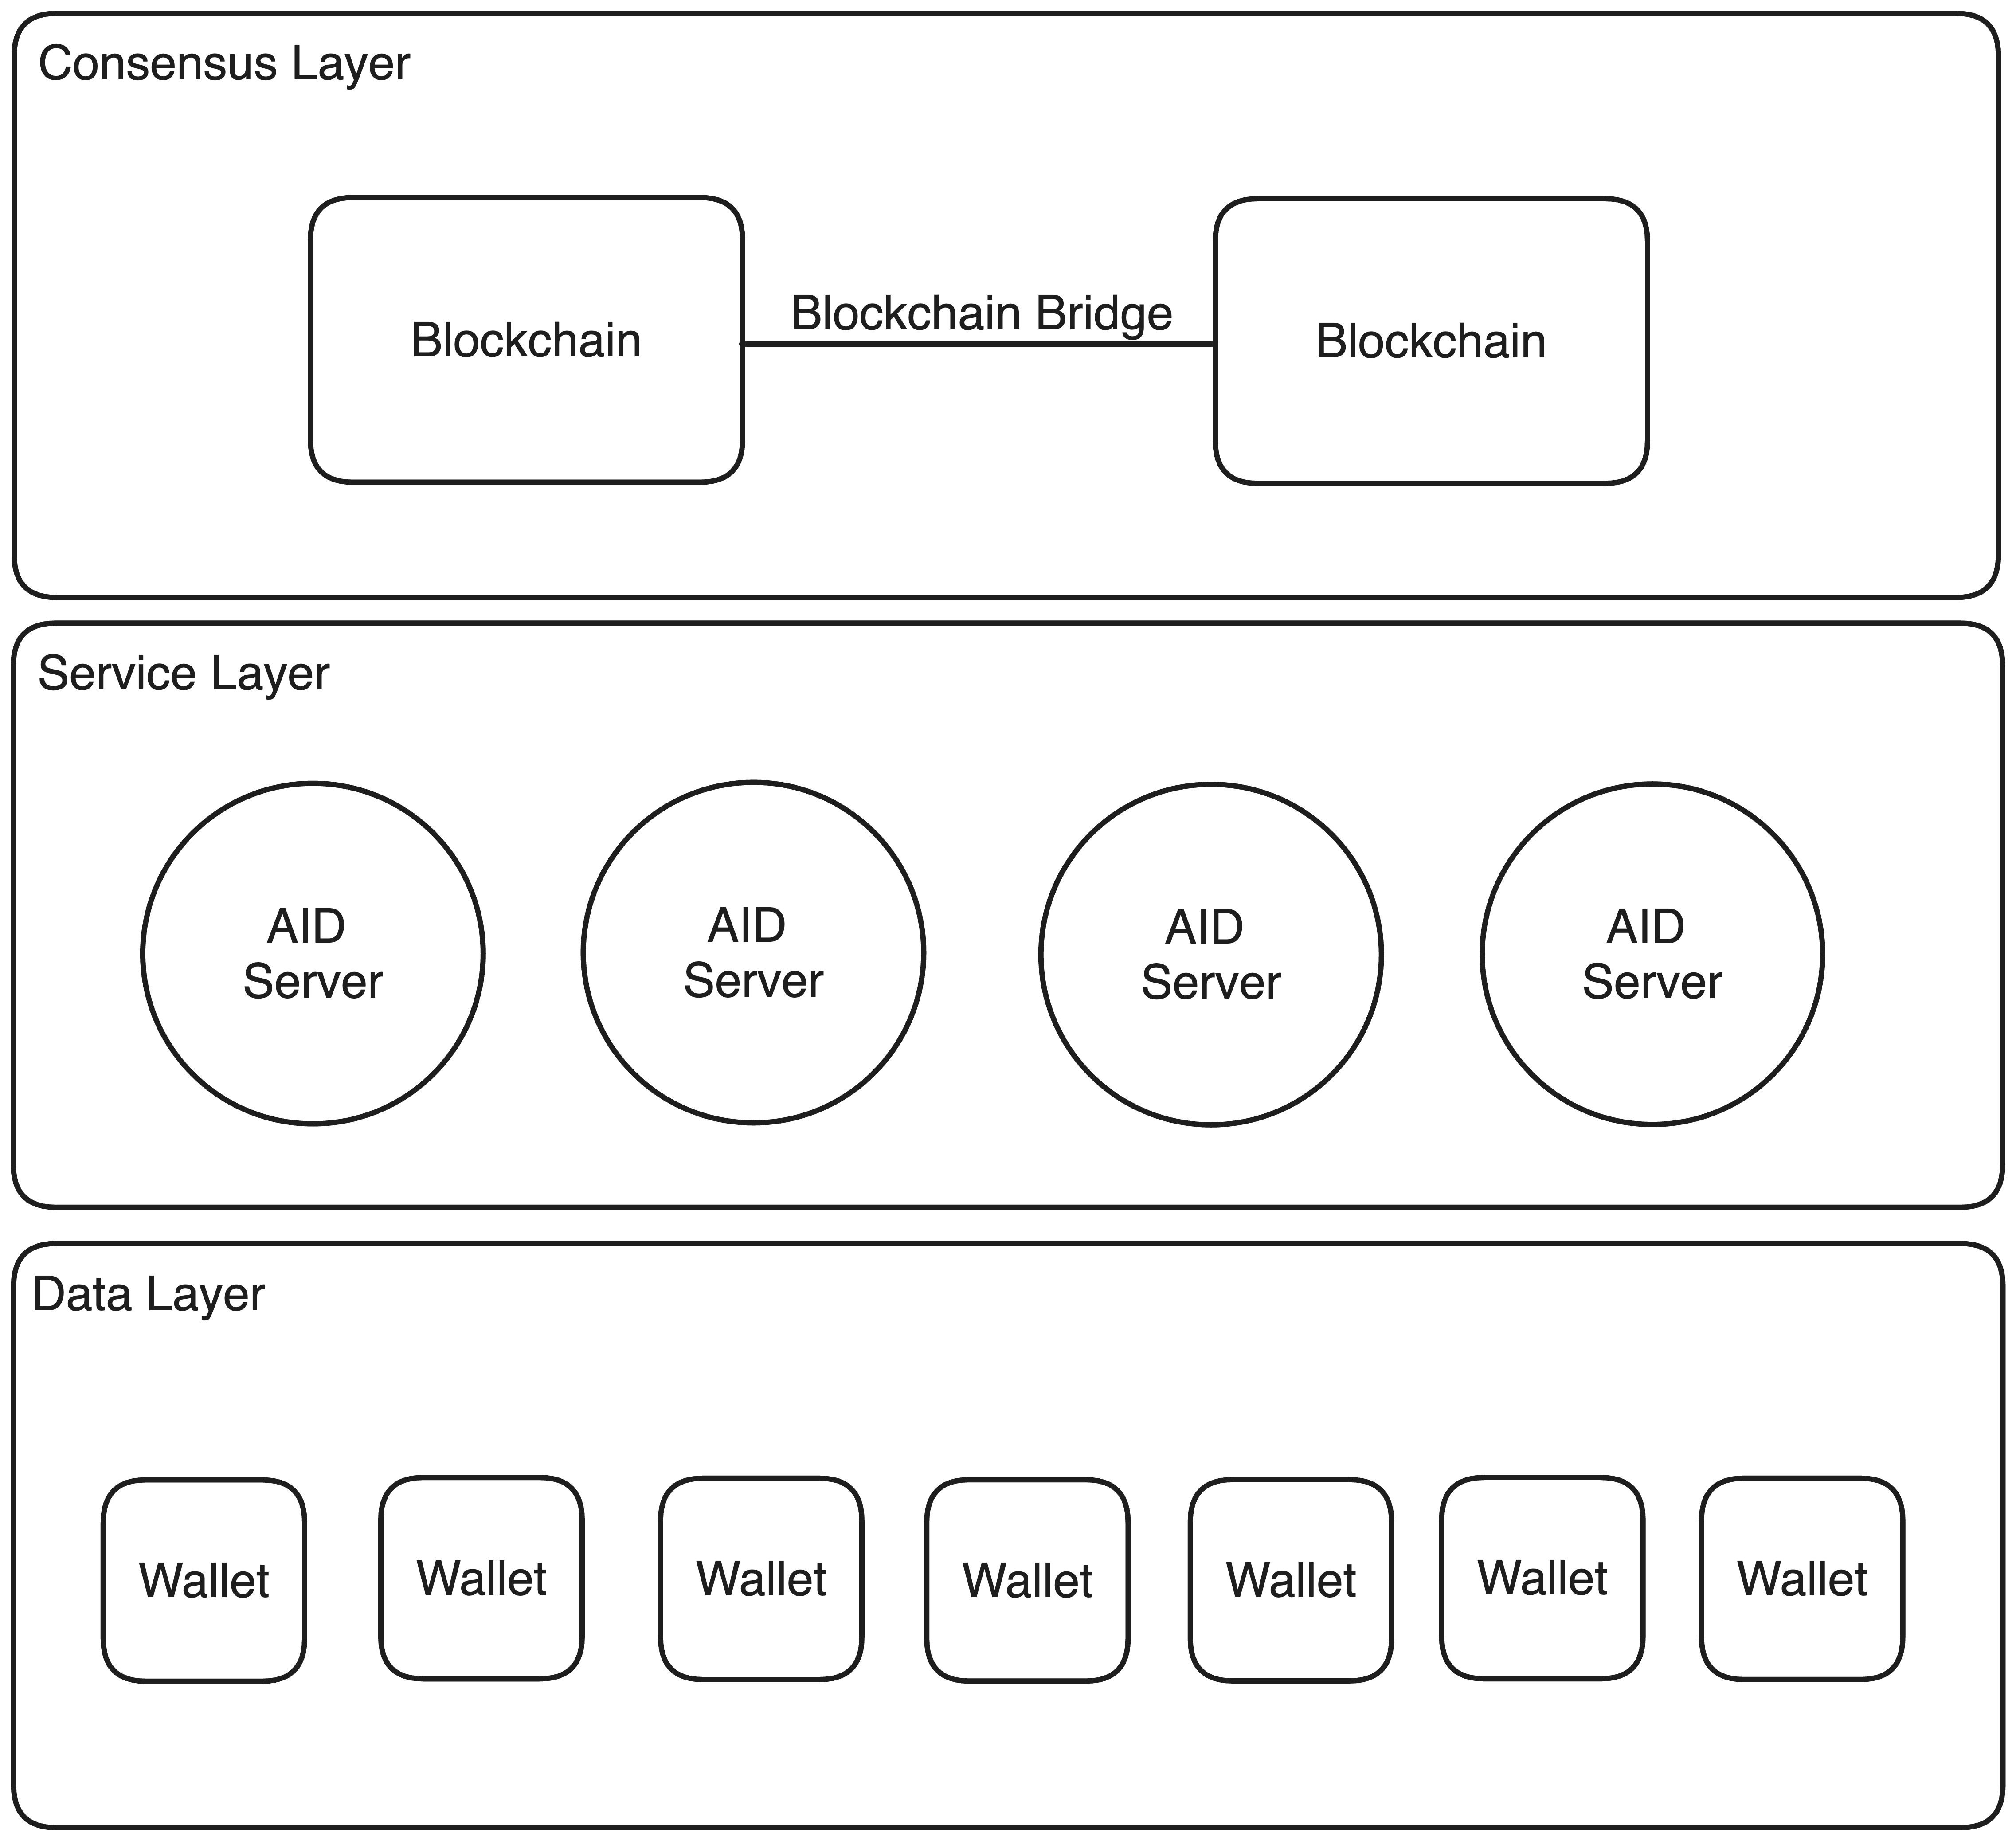
\includegraphics[width=0.8\textwidth]{figures/aidLayers.png}
  \caption{自主身份系統分層架構}
  \label{fig:aid-layers}
\end{figure}

更深入地看,共識層的核心組成是具備共識機制的區塊鏈系統。這一層級可通過跨鏈橋等先進機制實現水平擴展,顯著提升系統的可擴展性。區塊鏈中的智能合約扮演著關鍵角色,它為服務層和數據層提供了對共識數據進行讀寫操作的介面。值得注意的是,共識層的實現並不局限於區塊鏈技術。在存在可信第三方機構的情況下,其他形式的共識機制同樣可以被採用,這為系統設計提供了更大的靈活性。

服務層由多樣化且相互獨立的網路服務構成,這些服務可能以移動應用、網站或API服務等形式呈現。儘管各服務的具體需求可能大相徑庭,但它們都需要強大的身份管理功能。為了滿足這一普遍需求,我們提出了一個統一的解決方案:AID Server。我們設計了一個用於多種程式語言的後端SDK規格,它在保留客製化空間的條件下為服務提供者提供了一個標準化的身份管理介面。通過AID Server,服務開發者能夠輕鬆地實現與共識層和數據層的無縫對接,大大簡化了開發流程並維持了系統的一致性。

數據層主要由大量獨立的終端應用組成,這些應用可能是智能手機APP、個人電腦軟體或物聯網(IoT)設備等。與服務層類似,數據層中的應用雖然功能各異,但都需要可靠的身份管理能力。針對這一需求,我們設計了名為Wallet的前端SDK規格。Wallet能在多種程式語言下為應用開發者提供統一的身份管理介面。這使得開發者能夠輕鬆地實現數據層應用與共識層和服務層的有效對接,從而構建出一個完整且高效的生態系統。

這種多層架構設計不僅確保了系統各部分的模組化和解耦,還提高了整體系統的可擴展性、靈活性和安全性。通過標準化的介面和SDK規格,我們大大降低了開發難度,同時提高了不同層級間的互操作性。接著,我們將進一步介紹各層的的具體規格與設計細節。
\subsection{共識層}
共識層是自主身份系統的基礎建設,主要由無數個智能合約組成。並且,所有智能合約都應該包含以下四個功能,分別介紹:
\begin{itemize}
  \item \textbf{數據寫入:} 將特定格式的數據雜湊寫入區塊鏈,並提供即時的評價與狀態寫入功能。
  \item \textbf{數據讀取:} 讀取區塊鏈上特定數據的雜湊,並獲取相關評價與狀態資訊。
  \item \textbf{狀態更新:} 由證書擁有者執行,用於即時變更證書狀態,如撤銷或停用。
  \item \textbf{評價機制:} 允許用戶根據智能合約規則,以特定格式留下評價內容。
\end{itemize}
為了更好地理解共識層的運作,讓我們以學歷驗證為例。在這個場景中,用戶向學校申請學歷證明,學校將證明的數位簽名寫入區塊鏈。任何需要驗證該學歷的服務都可以通過讀取區塊鏈上的簽名來確認其真實性。若用戶的學歷狀態發生變化,學校可以即時更新區塊鏈上的簽名狀態,確保驗證方獲得最新資訊。此外,如果某企業對學歷證明的可信度存疑,可以在區塊鏈上留下評價,供其他驗證方參考。

為了保障用戶自主權,區塊鏈上寫入的簽名應遵循特定協議的智能合約,使用戶能自由決定操作簽名的規則。例如,用戶可以選擇具有刪除評價功能的智能合約來承載學歷證明的簽名,從而可以刪除特定的惡意評價。這種機制不僅保障了學歷資訊的即時性與真實性,還建立了一個動態且可自主控制的共識系統,大幅提升了身份管理系統的可靠性、效率及彈性。

然而,這樣的設計也面臨著諸多挑戰,首要問題是如何有效評價鏈上簽名,並將其轉化為影響用戶信譽的機制。其次,作為系統信任核心的區塊鏈,其長期穩定運營的可行性也是一個極需解決的問題。最後,在跨服務的用戶數據變化過程中,如何建立有效的共識機制同樣是一個關鍵議題。這些新架構下衍生的問題都需要深入探討和研究,以確保系統的可靠性和可持續性。

為了解決評價問題,我們必須理解為何在自主身份系統中,用戶需要在區塊鏈上的簽名留下評價。這涉及去中心化自治組織(DAO)的概念,我們可以將整個自主身份系統視為一個大型自治組織。在這個組織中,每個自主身份(AID)都是成員,每個成員都有信任和被信任的需求。傳統的中心化身份系統中,這種需求是由中心化的身份服務提供者來滿足的。而在自主身份系統中,這種需求則是通過區塊鏈上的評價來滿足。因此,我們可以將評價視為一種投票,其結果直接反映用戶的信譽。

值得注意的是,不僅用戶之間需要建立信任,用戶與服務之間也同樣需要。這種雙向信任的建立主要通過彼此評價來實現。因此,評價成為自主身份系統中的一個核心機制。評價機制的設計需要考慮諸多因素,如評價的權重、範圍和內容如何設定等。這些都涉及實際用戶的需求,我們希望保留用戶的自主權,讓他們可以自由選擇不同協議的智能合約作為區塊鏈上的評價機制。至於智能合約協議的協調與自治,我們期望能夠通過 DAO 中統治代幣的概念來實現。

作為系統信任核心的區塊鏈如何運營,這涉及到區塊鏈的經濟模型。我們提議在區塊鏈中發行一種逐漸增加的自主身份統治代幣。這種代幣可被抵押用於創建用戶的自主身份,藉此防止惡意用戶大規模創建惡意帳戶。每個自主身份(相當於其背後的代幣)可參與定期投票,討論評價機制的調整、新的智能合約協議等議題。為確保區塊鏈的長期運作,我們建議對失去信任的用戶實施懲罰,同時獎勵基礎設施的運作。因此,用於創建自主身份的代幣抵押後不可贖回,而是被鎖定在區塊鏈上。這樣可以確保用戶不會輕率創建自主身份,並激勵用戶維護自身自主身份的信譽。此外,我們建議對用戶在鏈上的每項操作採取使用者付費模式,使區塊鏈的維護者能獲得報酬,從而保證區塊鏈的持續運作。

最後,我們需要設計一個機制來實現跨服務的用戶數據變化共識。這是一個常見的網路服務需求,如微服務間的調用即為典型案例。在我們的設計中,資料的控制權從服務提供者轉移到用戶身上,這將大幅改變當前網路後端應用的設計。基於共識層的功能,我們提議讓用戶成為多個服務之間的橋樑。具體而言,用戶在區塊鏈外傳遞特定格式的資訊,而服務提供者則在區塊鏈上驗證這些資訊,從而達成共識。

舉例來說,在實作一個利用第三方支付服務的購票系統時,我們的方法與現行的網路後端設計有所不同。現有設計中,購票系統全權負責與支付體系的串接,用戶僅需與購票系統溝通。而在我們提出的架構下,流程如下:
\begin{enumerate}
  \item 購票系統要求用戶到銀行服務完成支付並取得收據。
  \item 銀行服務將收據的簽名寫入區塊鏈。
  \item 用戶向購票系統提交收據和購買請求。
  \item 購票系統在區塊鏈上驗證收據的真實性。
  \item 驗證通過後,完成購票流程。
\end{enumerate}
這種方式不僅確保了數據的可信度,還賦予了用戶更多對自身數據的控制權,體現了自主身份系統的核心理念。
\subsection{服務層}
服務層是自主身份系統的應用層,負責提供各種服務。自主身份系統不包含具體服務的實作,只是提供名為AID Server的後端SDK規格,讓服務開發者能夠輕鬆地把自己的應用接入自主身份系統。我們設計了AID Server的幾個關鍵功能:
\begin{itemize}
  \item \textbf{身份管理:} 提供服務註冊、登入、登出等基本身份管理功能。
  \item \textbf{證書管理:} 提供共識簽名的創建、更新、讀取、評價等功能。
  \item \textbf{數據管理:} 提供用戶數據的導入、導出等功能。
\end{itemize}
以下將分別介紹這幾個功能的設計細節。
\subsubsection{身份管理}
對服務提供者來說,一個新的自主身份想要註冊,必須要提供基於「自主證書機制」創建的證書。此時,服務提供者可以選擇是否接受這個新的自主身份。大多數的公開服務應該會接受任何自主身份,但私人服務可能會有更高的要求,例如只接受特定機構簽章的自主證書,又或是基於評價機制被足夠信任的自主身份。當服務提供者接受了一個新的自主身份,這個自主身份就可以開始使用服務了。

特別地方在於,自主。
\subsubsection{證書管理}
\subsubsection{數據管理}
\subsection{數據層}
數據層是自主身份系統的存儲層,負責存儲用戶個人數據。我們設計了名為Wallet的前端SDK規格,讓數據層應用開發者能夠輕鬆地把自己的應用接入自主身份系統。Wallet的幾個關鍵功能如下:
\begin{itemize}
  \item \textbf{身份管理:} 提供自主身份的註冊、驗證等功能。
  \item \textbf{數據管理:} 提供用戶數據的上傳、下載等功能。
  \item \textbf{證書管理:} 對共識簽名的更新、讀取、評價等功能。
  \item \textbf{數據存儲:} 儲存用戶的數據。
\end{itemize}
以下將分別介紹這幾個功能的設計細節。
\section{資料結構}
\subsection{AID Server}
\subsection{Wallet}
\subsection{Consensus Core}
\section{自主身份系統的威脅模型}
\section{本章小結}
系統如何解決所有缺點,並且保留所有優點。